\chapter{惯性辅助的单目视觉SLAM}

\section{基于预积分的惯性辅助定位}
\subsection{噪声模型}
\subsection{状态传递}
\subsection{观测模型}

\section{多传感器标定}

\section{单目视觉跟踪}

\section{集束优化}

目前绝大多数的SLAM算法通过集束优化\citep{triggs1999bundle}(Bundle Adjustment,BA)方法来对状态进行估计在传统的视觉SfM算法中,集束优化是指通过联合优化所有的视觉观测误差来同时求解最优的相机位姿状态和路标点状态的方法。而对于使用了更多传感器的SLAM系统,除了路标点和位姿状态,集束优化算法还需要实时地、持续对系统的其他状态比作出估计。对于视觉惯性SLAM,集束优化通常会通过联合优化所有的视觉观测和惯性观测来同时求解相机或IMU的位姿、速度以及IMU的bias状态。

\subsection{基于图优化的状态估计}

图优化方法是分析并求解SLAM后端状态估计问题的常用工具。最早在机器人领域,为了解决多段激光传感器数据额融合时的全局一致性问题,\citep{lu1997globally,lu1997robot}提出了基于位姿图的优化方法。\citeauthor{thrun2006graph}在此基础上进一步提出了GraphSLAM\citep{thrun2006graph},使用由位姿状态和路标点状态以及它们之间的约束构成的因子图来描述集束优化问题。因子图可以很直观地描述集束优化问题中状态和约束之间的关联,有助于分析集束优化问题的各种性质。经过长时间的发展,图优化方法已经成为SLAM领域的经典方法。

\begin{figure}[htbp]
    \centering
    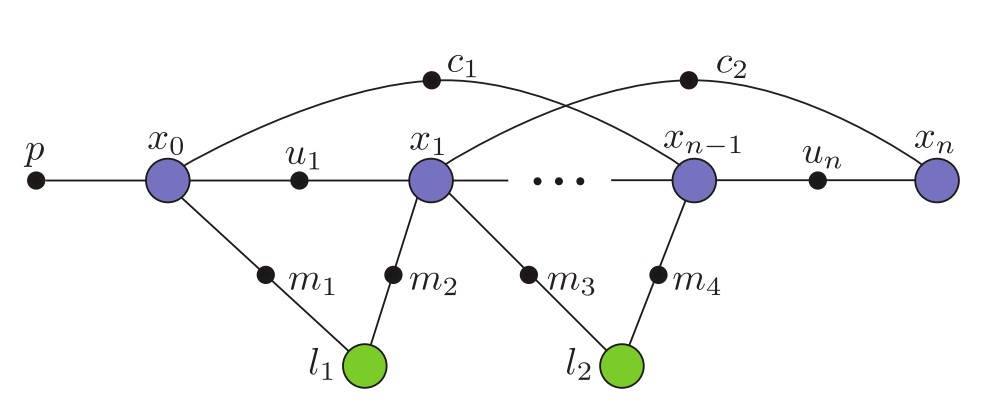
\includegraphics[width=.6\textwidth]{figs/factor_graph.png}
    \caption{因子图示例\citep{kaess2012isam2}:紫色节点代表位姿状态,绿色节点代表路标点状态,黑色节点代表状态之间的约束因子。}
    \label{fig:factor_graph}
\end{figure}

图\ref{fig:factor_graph}展示了一类常见的因子图结构。按照图示的例子,一个SLAM问题中可能存在的约束有状态变量的先验约束$p$,相邻状态之间的相对位姿约束$u_1 \dots u_n$,非相邻状态之间的回路闭合约束$c_1,c_2$以及视觉观测约束$m_1 \dots m_4$等。而求解完整集束优化的过程就相当于最大化整个因子图中的所有约束的集合$\mathcal{Z}$关于所有状态集合$\mathcal{X}$的联合条件概率:

\begin{equation}
    P(\mathcal{Z}|\mathcal{X}) = \prod_{f_i\in\mathcal{Z}} P(f_i(\mathcal{X}_i))
\end{equation}

其中$\mathcal{X}_i$代表所有与约束节点$f_i$相邻的状态节点。通常会假设这是一个高度非线性系统,并且所有的约束$f_i$的噪声服从高斯分布$f_i\sim\mathcal{N}(\mu_i, \sigma_i^2)$。这样的的概率最大化问题,无法通过线性的求解器直接求解状态集合$\mathcal{X}$的最优值,而需要先将其转化为非线性最小二乘问题,然后通过迭代求解的方式来解决:

\begin{equation}
\begin{aligned}
    \mathcal{X}^\ast &= \mathop{\arg\max}_{\mathcal{X}}
                        \prod_{f_i\in\mathcal{Z}} P(f_i(\mathcal{X}_i)) \\
                     &= \mathop{\arg\min}_{\mathcal{X}}
                        \sum_{f_i\in\mathcal{Z}} \frac{1}{2}
                        \lVert f_i(\mathcal{X}_i)) \rVert_{\sigma_i^2}^2
\end{aligned}
\end{equation}

\subsection{滑动窗口优化}

离线的SfM算法对实时性的要求不高,故一般会使用全局集束优化来求解所有状态的最优值。但在SLAM算法中,频繁求解完整的集束优化将会严重降低系统的性能,特别是当地图规模增长到一定程度后,完整集束优化的时间复杂度往往以至少立方的速度增长,这对于AR、自动驾驶等对实时性要求很高的应用是不可接受的。

与SfM算法不同,基于SLAM的应用往往更关心系统最新的位姿状态和路标点状态,而对历史状态的需求较低。针对这一情况,PTAM\citep{klein2007parallel}最早提出了区分局部优化和全局优化的架构。即使用一个前台线程负责快速求解一个规模较小局部集束优化,以快速获取最新状态的粗略估计;另外一个后台线程以更低的频率对所有状态进行全局集束优化,对状态估计问题进一步优化。这种设计既保证了前台状态估计的时间上限,又保证了全局状态的一致性,如今已经成为了SLAM系统主流设计思路。

\subsection{边缘状态估计}

\section{小结}
